%!TEX root = ../report.tex
\chapter{Background theory}
\label{cha:background_theory}
In this chapter, the theory for building search methods are explored. General graph theory is introduced, with algorithms for traversal of graphs. Different structures used in RDF graphs are discussed, and the technology used for traversal and search are explored.

\section{Graph theory}
Graphs are mathematical structures modeling relationships between objects, and the study of these structures is called graph theory. A graph consists of vertices, sometime called nodes, and connected by edges, \emph{G(V, E)}. A graph can take on different shapes, giving the graph special properties. By giving the edges a direction, the graph can take on further properties. In computer science the relationships in graphs make them suited for applications in many different fields, such as data mining, image segmentation, networking and more \cite{riaz2011applications}. 

A graph where the edges have a direction is called a directed graph as seen in figure \ref{fig:DAG}. Here the vertices are connected to each other, with an arrow displaying the direction. An example of an undirected graph can be seen in figure \ref{fig:DAGvsAG}. In both types of graphs, a vertex can have multiple edges. Graphs can contain cycles, meaning that vertices are connected to each other so that it is possible to follow edges in such a way that it leads back to the initial vertex. An example of such a cyclic graph can be seen in figure \ref{fig:DAGvsDG}. Acyclic graphs have an inherent topological ordering. This ordering makes it easy to find properties in the graph, such as the shortest path between two vertices.

\begin{figure}
    \centering
    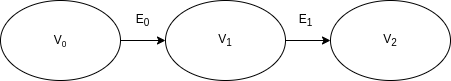
\includegraphics[scale=0.5]{figs/simpleDAG.png}
    \caption{Simple Directed graph.}
    \label{fig:DAG}
\end{figure}

\begin{figure}
    \centering
    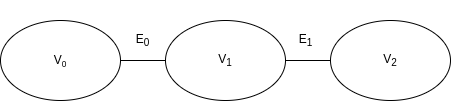
\includegraphics[scale=0.5]{figs/simpleAG.png}
    \caption{Example of non-directed graph.}
    \label{fig:DAGvsAG}
\end{figure}

\begin{figure}
    \centering
    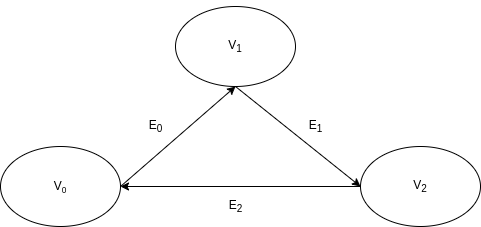
\includegraphics[scale=0.5]{figs/triangleDG.png}
    \caption{Directed graph with a cycle.}
    \label{fig:DAGvsDG}
\end{figure}

\subsection{Graph traversal}
When traversing a graph, two methods are commonly used, breadth first and depth first. Both traversal methods need a starting point. If there is no natural starting point or root, any vertex in the graph can be selected. Breadth first traversal use a queue containing vertices in the order they are discovered. From the start vertex, all connected vertices are added do the queue, then the first vertex in the queue is visited, and explored. Vertices connected to the current node is added to the back of the queue, so that the oldest discovered node is the next to be visited. In contrast a depth first search will add newly discovered vertices to the front, so that the newly discovered vertex will be visited next.

Both traversal methods can be used on directed and undirected graphs. On an undirected graph, any vertex discovered can be added to the list of vertices to visit. In a directed graph, only vertices connected by an edge with a direction going from the current vertex, and to another vertex will be followed. Both traversal types can have a termination condition, so that the traversal will stop before traversing the entire graph.

\begin{algorithm}
    \caption{Breadth first traversal exploring entire graph}
    \label{BFT}
    \SetAlgoLined
    \KwResult{List of vertices in the order traversed}
    Start vertex $V_r$\; Array $\mathbf{Q}$ Add($V_r$)\; List $l$\;
    \While{$\mathbf{Q} \neq \emptyset$}{
        $v$ = $\mathbf{Q}$ GetFirstElement()\;
        \If{v not discovered}{
            $v$ setDiscovered\;
            $n$ = GetAllConnectedVertices($v$)\;
            $\mathbf{Q}$ Add($n$)\;
            $l$ Add($v$)\;
        }
    }
    \Return{$l$}\;
\end{algorithm}

\begin{algorithm}
    \caption{Depth First traversal exploring entire graph}
    \label{DFT}
    \SetAlgoLined
    \KwResult{List of vertices in the order traversed}
    Start vertex $V_r$\; Array $\mathbf{S}$ Add($V_r$)\; List $l$\;
    \While{$\mathbf{S} \neq \emptyset$}{
        $v$ = $\mathbf{S}$ GetLastElement()\;
        \If{v not discovered}{
            $v$ setDiscovered\;
            $n$ = GetAllConnectedVertices($v$)\;
            $\mathbf{S}$ Add($n$)\;
            l Add($v$)\;
        }
    }
    \Return{$l$}\;
\end{algorithm}

Algorithm \ref{BFT} and \ref{DFT} are very similar. Both algorithms explore an entire graph from a root vertex R and returns a list of vertices in the order they are traversed. The main difference between breadth first and depth first is how the next vertex to visit is selected. If we use the graph in figure \ref{fig:graph} as an example, we can see that the vertices are numbered 0 to 6, and the graph have one cycle. Using breadth first the result is a list with the vertices in order from 0 to 1, the paths selected is seen in figure \ref{fig:BFT}. Using depth first traversal, the order and paths are different, as seen in figure \ref{fig:DFT}. The order in depth first would be 0, 2, 6, 5, 1, 4, 3, assuming the left most vertex is the first to be added.

\begin{figure}
    \centering
    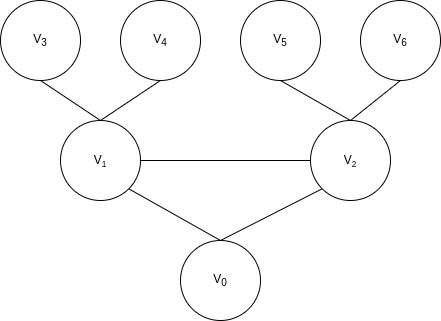
\includegraphics[scale=0.5]{figs/Graph.png}
    \caption{Graph with one cycle}
    \label{fig:graph}
\end{figure}

\begin{figure}
    \centering
    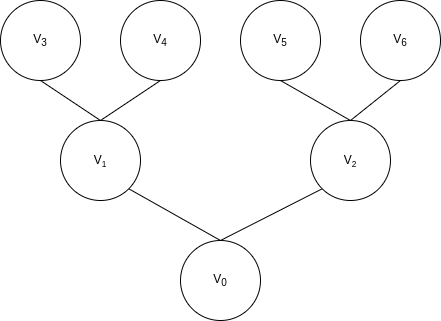
\includegraphics[scale=0.5]{figs/BFT.png}
    \caption{Breadth first traversal of graph \ref{fig:graph}}
    \label{fig:BFT}
\end{figure}

\begin{figure}
    \centering
    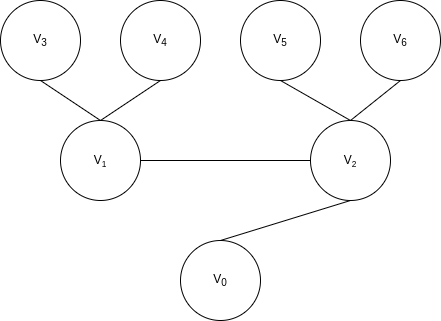
\includegraphics[scale=0.5]{figs/DFT.png}
    \caption{Depth first traversal of graph \ref{fig:graph}}
    \label{fig:DFT}
\end{figure}

Building on the breadth first traversal, it is possible to create an algorithm for finding a minimum spanning tree. In algorithm \ref{MinTreeBFS} this is done, while also adding a termination condition. The algorithm terminates when a set of terms have been discovered in the graph and returns the minimum spanning tree contains all the terms. This algorithm assumes the vertices are objects containing a list of connected nodes.

\begin{algorithm}
    \caption{Minimum spanning tree with breadth first search}
    \label{MinTreeBFS}
    \SetAlgoLined
    \KwResult{Minimum tree containgin terms $T_q$}
    Root vertex $V_r$\; Terms $T_q$\; Array $\mathbf{Q}$ Add($V_r$)\; Minimum tree $M_t$\; MatchedTerms $T_m$\;
    \While{$\mathbf{Q} \neq \emptyset$}{
        $v$ = GetFirstElement($\mathbf{Q}$)\;
        $M_t$ Add($v$)\;
        \If{$v$ GetTerms $\subseteq T_q$}{
            $T_m$ Add($v$ GetTerms $\cap T_q$)\;
        }
        \If{$T_q$ = $T_m$}{
            Break\;
        }
        $n$ = GetNeighbors($v$)\;
        $\mathbf{Q}$ Add($n$)\;
    }
    \Return{$M_t$}
\end{algorithm}

\section{RDF, ontologies, and knowledge graphs}
Knowledge base, ontology and knowledge graph are terms with multiple definitions, and are often used interchangeably. The definitions here are used to clarify what they mean in this thesis and is not a definitive definition.

\subsection{Ontology}
Ontologies contain representations, conceptualization, relations, categorization, and formal naming of data \cite{davies2006semantic}. Ontologies allows for semantic modeling of knowledge. Here knowledge is data that is not ordered in a strict structure. Using ontologies allows data to be better structured, and reason about the semi-structured data. Ontologies also have its own language, called the ``web ontology language'' or OWL. This language was created to standardize ontologies.

Using the structure of ontologies makes it possible interpret natural language \cite{cimiano2014ontology}. Here the ontology gives meaning to the words, based on the classes and relations in the ontology. Building on the meaning given to words from the ontology, it is possible for a computer to infer meaning from a sentence or set of words.

\subsection{RDF as knowledge graphs}
Structuring an ontology using a framework like RDF creates a knowledge graph. There is no clear definition on exactly what constitutes a knowledge graph. A broad definition of knowledge graph is ``A knowledge graph acquires and integrates information into an ontology and applies a reasoner to derive new knowledge'' \cite{KGDef}. This definition encompasses multiple technologies. Another definition using RDF graphs as a bases is ``We define a Knowledge Graph as an RDF graph. An RDF graph consists of a set of RDF triples where each RDF triple (s, p, o) is an ordered set of the following RDF terms: a subject s $\in$ U $\cup$ B, a predicate p $\in$ U, and an object U $\cup$ B  L. An RDF term is either a URI u $\in$ U, a blank node b $\in$ B, or a literal l $\in$ L'' \cite{KGDefYago}. This latter definition is how knowledge is structured in the data used in this thesis.

Using RDF as a format when modeling knowledge makes it possible to create structured content from semi-structured knowledge. This structure makes knowledge usable for computers, where it previously would have been difficult to extract accurate and exact knowledge. This information can then be presented in a human readable fashion, or it can be used in other fields, like artificial intelligence.

When structuring knowledge from other content it is divided into small packets of information, where one such packet represents a single fact. In RDF facts are represented as triples. Each triple has a subject that the fact is describing. These subjects are called entities, and a single entity can have any number of facts. Entities are linked together through facts, forming the graph. When linking entities, both vertices must be URIs.

In the RDF graph each triple consists of a subject, object, and a predicate. Some entities can be present in multiple languages, or there can be different names for a single entity. This creates a special case, where a single entity can be described by multiple subjects. In such cases, the subject identifies an entity, alias for the entity, or other variation of an entity, and the subject can then have relations to main vertex describing the entity.

Predicates are always a URI. URIs used for predicates differ from the ones used for subjects and objects in that predicates are connected to specific types. A type is an identifier used to describe what the relation between the subject and object represents. Predicates can also be treated as a subject in a triple, which is used to give special properties, types, and classes to predicates.

Objects have the widest range of possible entries. Like subjects and predicates, objects can be URIs. Object URIs can be entity identifiers like subjects, they can be class identifiers, they can contain some data and a data type, or they can be blank. Blank vertices are vertices without any data or connections other than connections pointing to the blank vertex. Literals are vertices containing an atomic value. Atomic values can be defined by the user, so that literals can hold virtually any type of data. A literal can only have edges from other vertices, just like blank vertices.

\subsection{Existing knowledge graphs and ontologies}
Currently two of the largest open knowledge graphs are YAGO and DBPedia. Both these projects use information from Wikipedia to create the graph but differ in the ontology used to build the graphs. Yago also includes data from WordNet and GeoNames to accurately assign entities to classes. Both projects use RDF triples to create a knowledge graph.

\subsubsection{YAGO}
YAGO is an acronym for Yet Another Great Ontology and is the main data source in this thesis. The project describes itself as a knowledge base \cite{yago} and an ontology \cite{mahdisoltani:hal-01699874}, but is often described as a knowledge graph by others. In this paper YAGO is described as a knowledge graph. YAGO use automated information extraction from Wikipedia to create its knowledge graph. This graph is supplemented with data from WordNet, and GeoNames.

An example of YAGO entities can be seen in figure \ref{fig:Elvis}. From this example we can see that Elvis acted in Flaming Star on the 20th of December 1960. We can also see that Bobby Darin and Elvis is connected through the lifetime achievement award, and that Bobby Darin was borne in New York. New York also have coordinates connected to the node, rooting the vertex to a real place, but this is not present in the figure. In this example, only a small portion of the edges and vertices connected to the entities are displayed.

YAGO uses vertices for storing both spatial and temporal data. For temporal vertices unique predicates \cite{yago} are introduced. Temporal vertices use the ``xsd:date'' and ``xsd:dateTime'' data types. Both types follow the ISO 8601 format, YYYY-MM-DD, and introduces \# as a wildcard symbol. A fact can only hold a single time point and uses yagoDate as an extension of the xsd types \cite{yago}. In a date fact, the object holds the date information, and the predicate describes a connection between subject and date. In figure \ref{fig:Nidaros} we can see the triple ``Nidaros\_Cathedral wasCreatedOnDate 1300-\#\#-\#\#''. In this example the predicate wasCreatedOn is used to describe a relation between the subject and a date.

\begin{figure}
  \centering
  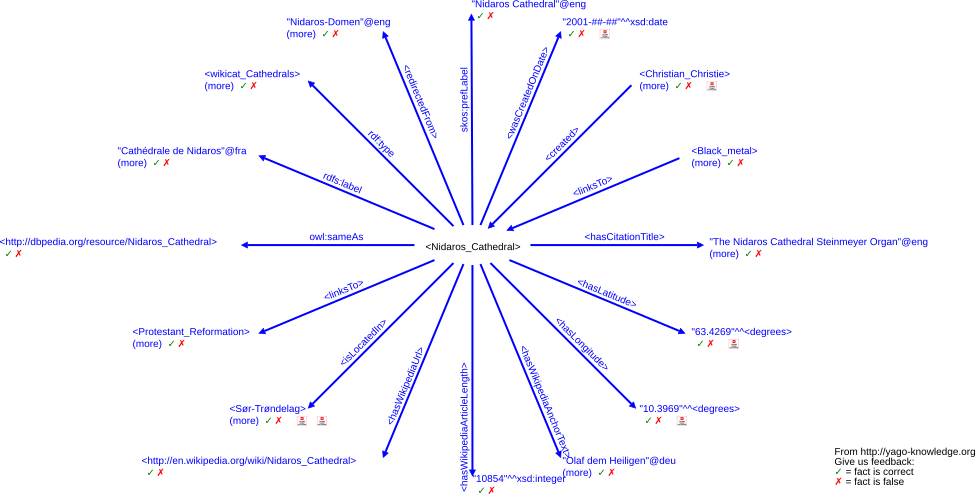
\includegraphics[scale=0.5]{figs/Nidaros_Cathedral.png}
  \caption[Nidaros cathedral as a subject in YAGO]{Nidaros cathedral as a subject in YAGO\protect\footnotemark}
  \label{fig:Nidaros}
\end{figure}

To describe a time span two facts are required. One of the facts describes a start date, and the second an end date. Since an entity can have multiple date facts connected, all date predicates are also assigned to a class. Start dates are assigned to a predicate with a type that has a ``creation'' class, such as ``StartedOnDate''. End dates are assigned to ``destruction'' type predicates. This makes it possible to deduce a time span for a given subject and predicate combination \cite{yago}.

Yago only contains permanent spatial data for entities on earth. This means that entities like cities, buildings, rivers and mountains are given a spatial dimension. In addition, events, people, groups and artifacts can be given a spatial dimension by relating the entity to a specific place. Using this transitive relation to the spatial fact, many entities can be related to a single spatial fact. All spatial facts must have a predicate that fall under the yagoGeoEntity class, and all objects used in a fact with a yagoGeoEntity must have a relation containing both ``hasLatitude'' and ``hasLongitude''.

\footnotetext{https://gate.d5.mpi-inf.mpg.de/webyago3spotlx/SvgBrowser?entityIn=\%3CNidaros\_Cathedral\%3E\&codeIn=eng}

\begin{figure}
  \centering
  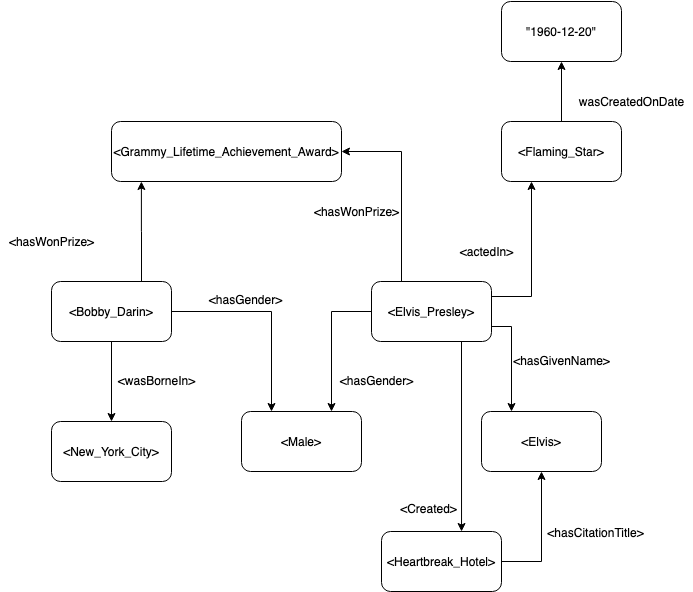
\includegraphics[scale=0.5]{figs/yagoExample.png}
 \caption{Connections in Yago around Elvis}
 \label{fig:Elvis}
\end{figure}
 
\subsubsection{DBPedia}
DBPedia is a crowd sourced knowledge graph using Wikimedia data\footnote{https://wiki.dbpedia.org/about}. This differs from YAGO, which is automated. Like YAGO, DBPedia use RDF for linking facts and entities, both contain facts in multiple languages, and have spatial and temporal data. With open data, and quarriable using SPARQL the data is easily available for anyone. DBPedia have multiple domains for spatial data, based on what type of spatial data it is. This includes coordinates, addresses, elevation, and many more, all creating a rich taxonomy.

\subsection{Uses for knowledge graphs}
One common use of knowledge graphs is to create an info box in search engines with data related to the search input. This information is a compact set of facts that tries to fit the search query. Because of the graph structure of knowledge graphs the information in the info box can be adapted to the query by choosing the predicates and related facts closest related to the query. This makes it possible to create a set of information that can give the user a quick overview of the information retrieved by the query.

Knowledge graphs are also used in machine learning \cite{nickel2015review}. Here models are trained on large knowledge graphs, and then used to predict new facts. When predicting new facts, the model predicts new edges in the graph between existing vertices. Another use of knowledge graphs is IBM Watson \cite{ferrucci2010building}. This project used many different knowledge graphs, among them YAGO and DBPedia, to beat humans in the game Jeopardy. Watson combined artificial intelligence, and natural language processing with the knowledge graphs to be able to accomplish this. Knowledge graphs have also been used to create recommendation systems \cite{oramas2016sound}. By combining data describing musical and sound items with links and entities from DBPedia and WordNet the recommendation system could use the graph to find new items that would be recommended. 

\subsection{Jena}
Apache Jena is a framework for working with semantic web and linked data like RDF. The framework contains tools for SPARQL querying, a query language made specifically for RDF graphs. Jena also contains REST-style SPARQL endpoints making the RDF data easily accessible. Using the existing standards makes it easy to use existing data sets, such as YAGO or DBPedia, and build utility on top of that data using some of the tools Jena provides.

Jena provides a persistent triple storage solution called TDB\footnote{https://jena.apache.org/documentation/tdb/architecture.html}. This storage contains tables for vertices called node table, indexing of triples, and a prefix table. The node table stores the representation of RDF ``terms'', where terms are any vertex, excluding some literals. Excluded literals are the xsd:decimal, xsd:integer, xsd:dateTime, xsd:date, and xsd:boolean types. Each vertex is stored with an ID used when data is loaded, and when querying constant terms. Node to ID mappings are stored as a B+ tree, while the ID to node mappings are stored as a sequential access file. Triples are stored in the triple table as a tuple containing three node IDs. The prefix table is used for supporting mappings that are used mainly for serialization of triples. Queries in Jena are run using ARQ, a SPARQL supported query engine.

\glsresetall